

\begin{frame}{Wikimedia Open Science Fellowship}

  %% - picture of the current fellows
  \begin{figure}
    \centering
    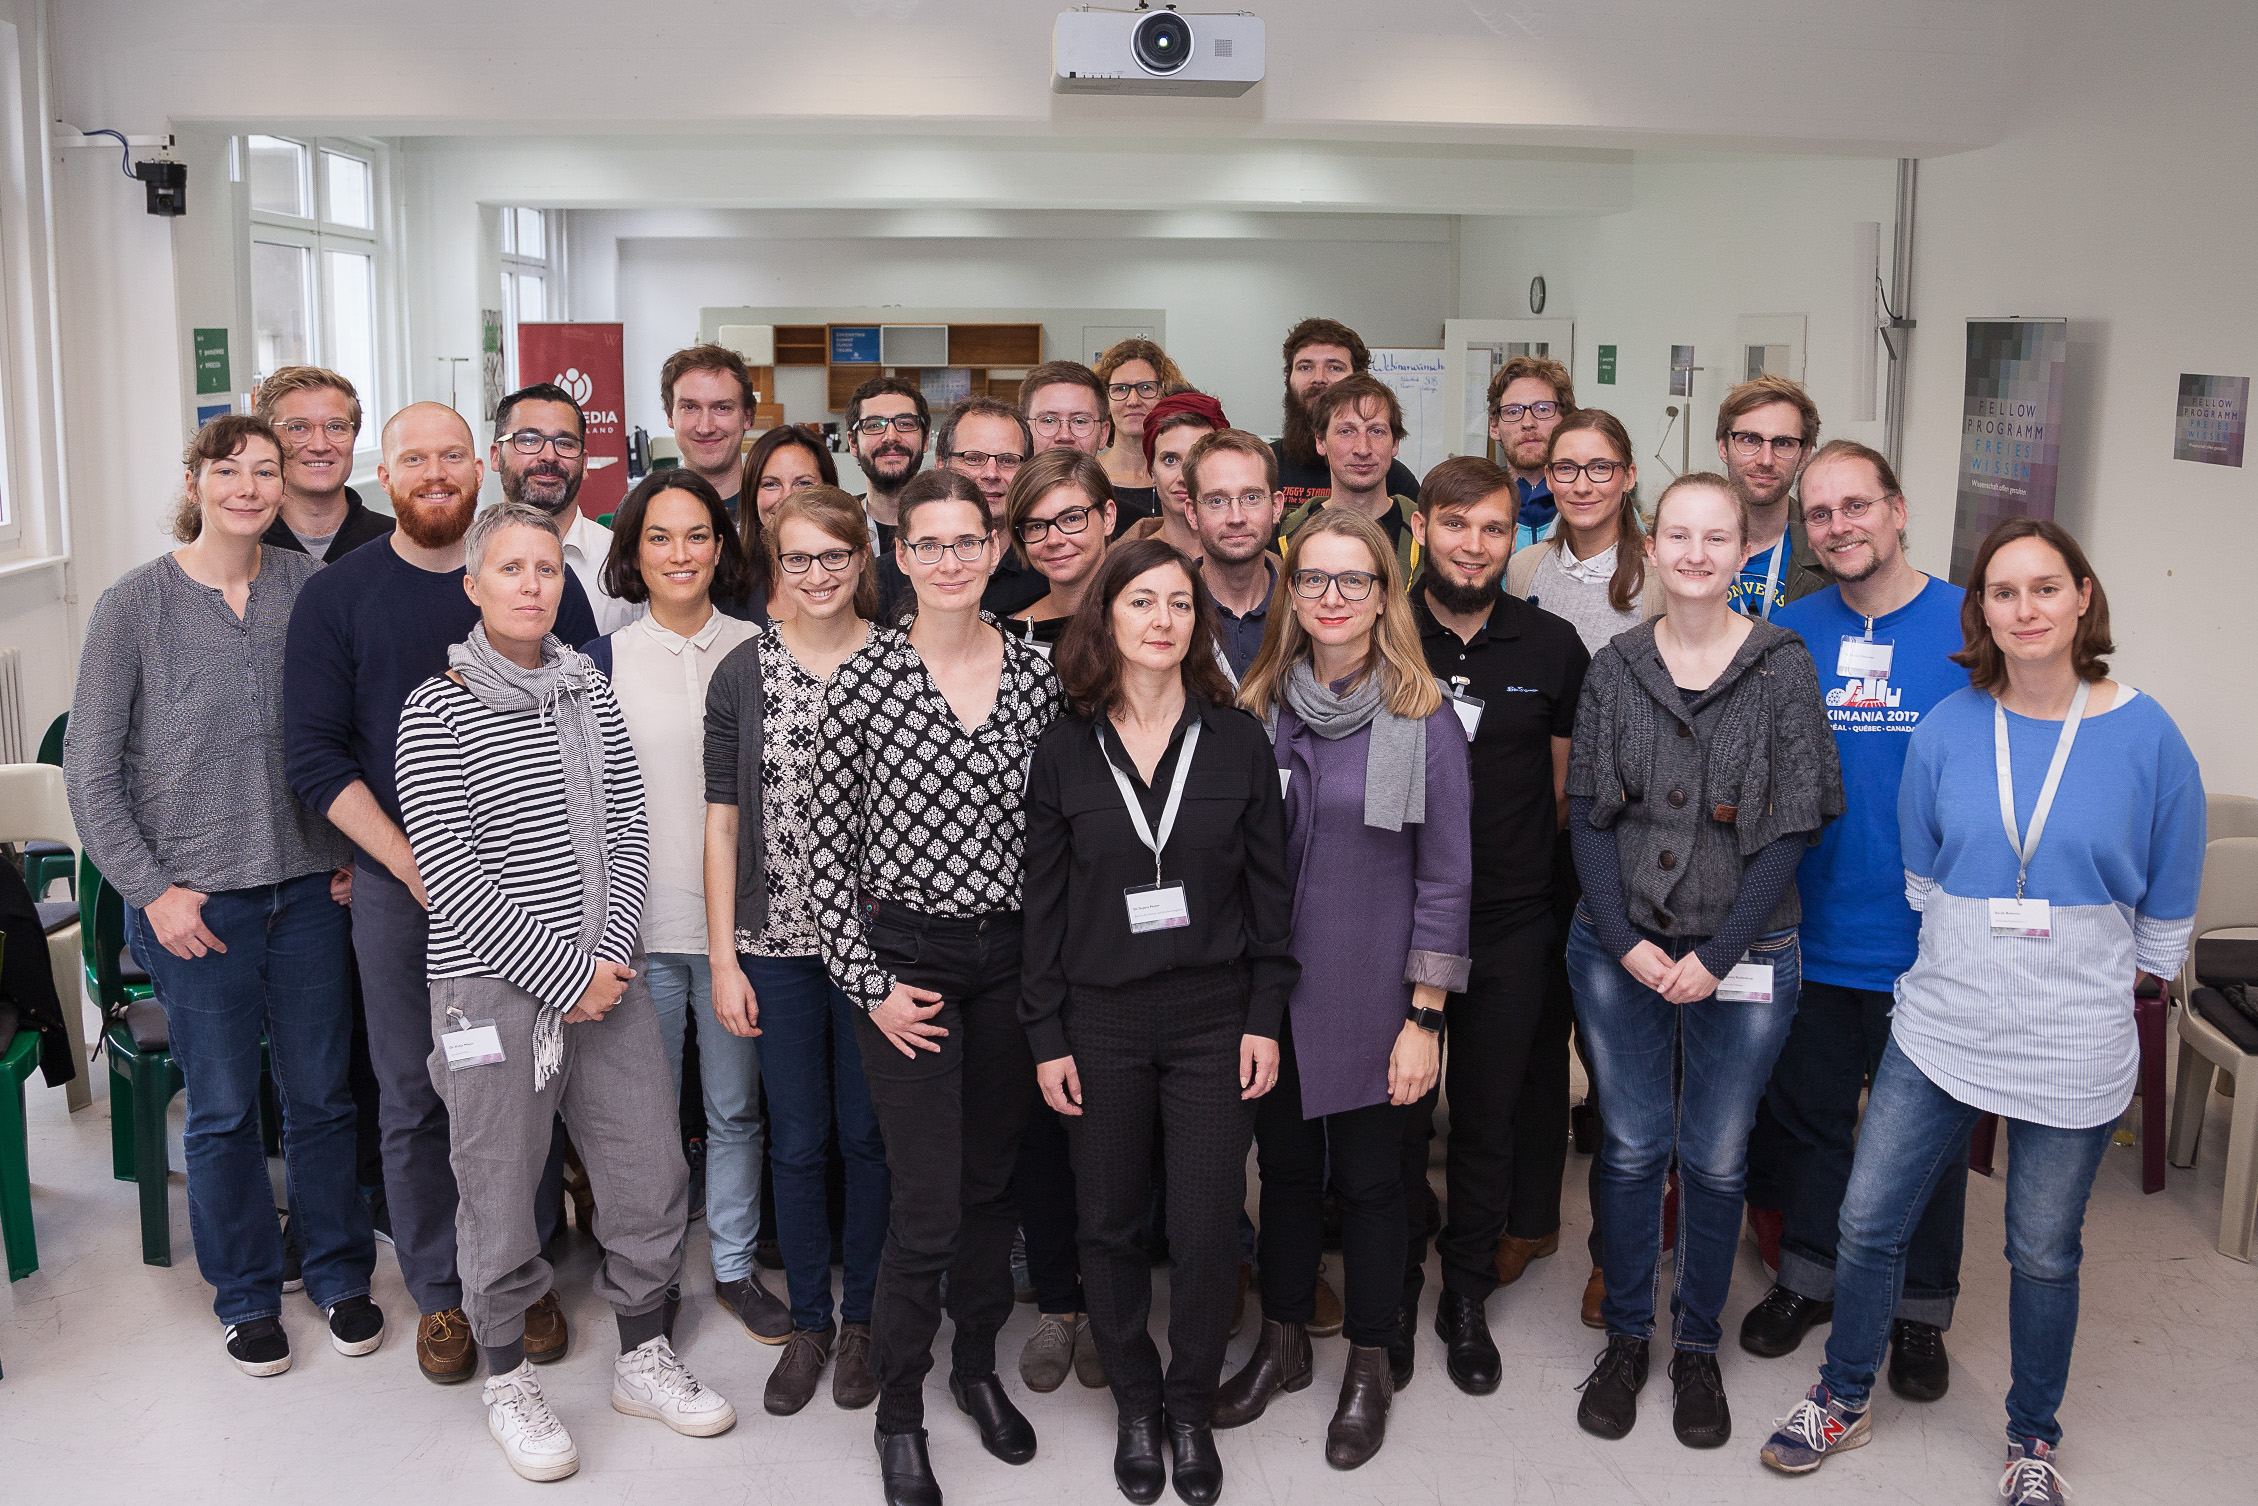
\includegraphics[width=0.875\textwidth]{%
    img/WOSF2017.jpg} %
  \end{figure}
  

  \source{\tiny Photo: Ralf Rebmann, CC BY-SA 4.0}


\end{frame}




\begin{frame}{Wikimedia Open Science Fellowship}

  % 
  \begin{columns}
    %
    \begin{column}{.55\textwidth}


      \begin{figure}
        \centering
        
\includegraphics[width=0.96\textwidth]{%
        img/logo_wosf_full.png} %
      \end{figure}
      

      
      

    \end{column}
    %
    \begin{column}{.45\textwidth}
      \minipage[c][0.625\textheight][s]{\columnwidth}

      \vspace{0.2cm}
      
      \begin{itemize}[leftmargin=*]

      \item[-] runs from October to June

      \item[-] fellows are paired with a mentor who supports the progress

      \item[-] financial support offered

      \item[-] program in German

      \item[-]       application for 3rd round now open!
      \href{http://bit.ly/osfprog}{bit.ly/osfprog}


      \end{itemize}

      

      \endminipage      
    \end{column}
  \end{columns}
  
\end{frame}

